\documentclass{standalone}
\usepackage{amsmath}
\usepackage{graphicx}
\usepackage{overpic}
\usepackage{tikz}

\begin{document}

	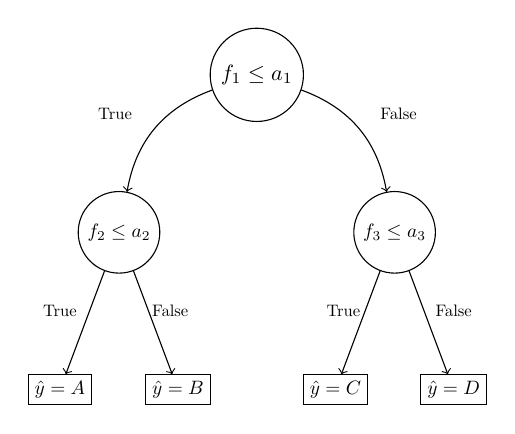
\begin{tikzpicture}
	\usetikzlibrary{graphs}
	\usetikzlibrary{backgrounds}

		
	\node [name=master,draw,circle,black,scale=0.8] at (0,3) {$f_1 \le a_1$};

	
	\node [name=run1,draw, circle, black, scale=0.7] at (-1.75,1) {$f_2 \le a_2$};

	\node [name=run2,draw, circle, black, scale=0.7] at (1.75,1) {$f_3 \le a_3$};
	
	
	\node [name=leaf1,draw, rectangle, black, scale=0.7] at (-2.5,-1) {$\hat{y}=A$};
	\node [name=leaf2,draw, rectangle, black, scale=0.7] at (-1,-1) {$\hat{y}=B$};
	\node [name=leaf3,draw, rectangle, black, scale=0.7] at (1,-1) {$\hat{y}=C$};
	\node [name=leaf4,draw, rectangle, black, scale=0.7] at (2.5,-1) {$\hat{y}=D$};


\node [scale=0.6] at (-1.8,2.5){True};
\node [scale=0.6] at (1.8,2.5){False};

\node [scale=0.6] at (-2.5,0){True};
\node [scale=0.6] at (-1.1,0){False};
\node [scale=0.6] at (1.1,0){True};
\node [scale=0.6] at (2.5,0){False};


\graph {(master)-> [bend right]{(run1)}};
\graph {(master)-> [bend left]{(run2)}};	
	
\graph {(run1)->{(leaf1),(leaf2)}};
\graph {(run2)-> {(leaf3),(leaf4)}};	
	
	
	

	\end{tikzpicture}
\end{document}